% =====================================================================
%  Catalytic Ladder Propagation
%
%  A federated retrieval architecture for catalysis data in which the
%  ladder is applied as a stencil over fetched records, and the primary
%  output is a verdict rather than an answer set.
%
%  Self-contained: every construction is derived here.
% =====================================================================
\documentclass[11pt,a4paper]{article}

\usepackage[utf8]{inputenc}
\usepackage[T1]{fontenc}
\usepackage{lmodern}
\usepackage[a4paper,margin=2.4cm]{geometry}
\usepackage{amsmath,amssymb,amsthm,mathtools}
\usepackage{bm}
\usepackage{booktabs}
\usepackage{array}
\usepackage{longtable}
\usepackage{enumitem}
\usepackage{microtype}
\usepackage{xcolor}
\usepackage{graphicx}
\usepackage{listings}
\usepackage{caption}
\usepackage{float}
\usepackage[round,sort&compress]{natbib}
\usepackage[colorlinks=true,linkcolor=blue!45!black,
            citecolor=blue!45!black,urlcolor=blue!45!black]{hyperref}
\usepackage[capitalise,noabbrev]{cleveref}

\captionsetup{font=small,labelfont=bf}

% ---- theorem environments ----
\newtheoremstyle{thmstyle}{\topsep}{\topsep}{\itshape}{}{\bfseries}{.}{.5em}{}
\theoremstyle{thmstyle}
\newtheorem{theorem}{Theorem}[section]
\newtheorem{lemma}[theorem]{Lemma}
\newtheorem{proposition}[theorem]{Proposition}
\newtheorem{corollary}[theorem]{Corollary}
\theoremstyle{definition}
\newtheorem{definition}[theorem]{Definition}
\newtheorem{axiom}[theorem]{Axiom}
\newtheorem{construction}[theorem]{Construction}
\newtheorem{principle}[theorem]{Principle}
\newtheorem{example}[theorem]{Example}
\theoremstyle{remark}
\newtheorem{remark}[theorem]{Remark}
\newtheorem{observation}[theorem]{Observation}

\crefname{axiom}{Axiom}{Axioms}
\Crefname{axiom}{Axiom}{Axioms}
\crefname{principle}{Principle}{Principles}
\Crefname{principle}{Principle}{Principles}

% ---- listings ----
\definecolor{kw}{RGB}{30,64,175}
\definecolor{cmt}{RGB}{22,101,52}
\definecolor{strc}{RGB}{159,18,57}
\definecolor{lstbg}{RGB}{250,250,250}
\lstset{
  basicstyle=\ttfamily\footnotesize,
  keywordstyle=\color{kw}\bfseries,
  commentstyle=\color{cmt}\itshape,
  stringstyle=\color{strc},
  backgroundcolor=\color{lstbg},
  frame=single,framesep=4pt,xleftmargin=6pt,xrightmargin=4pt,
  breaklines=true,showstringspaces=false,columns=fullflexible,tabsize=2,
  morekeywords={plan,from,fetch,require,translate,ladder,rung,medium,
    ambient,depleted,exchange,observe,role,direction,verdict,refuse,
    when,budget,within,emit,let,source,capability,toward,target}
}

% ---- notation ----
\newcommand{\Real}{\mathbb{R}}
\newcommand{\Nat}{\mathbb{N}}
\newcommand{\Gph}{\Gamma}
\newcommand{\med}{\mathsf{m}}
\newcommand{\flo}{\beta}
\newcommand{\cut}{\partial}
\newcommand{\sepc}{\sigma}
\newcommand{\pow}{\pi}
\newcommand{\Lad}{L}
\newcommand{\Tot}{\Omega}
\newcommand{\circu}{\varrho}
\newcommand{\unif}{\upsilon}
\newcommand{\Sspace}{\mathcal{S}}
\newcommand{\Sk}{S_{\mathrm{k}}}
\newcommand{\St}{S_{\mathrm{t}}}
\newcommand{\Se}{S_{\mathrm{e}}}
\newcommand{\kB}{k_{\mathrm{B}}}
\newcommand{\vans}{\textsf{answer}}
\newcommand{\vempty}{\textsf{empty}}
\newcommand{\vexp}{\textsf{unexpressed}}
\newcommand{\vsurf}{\textsf{unsupported}}
\newcommand{\vstarve}{\textsf{starved}}
\newcommand{\vhaust}{\textsf{exhausted}}
\newcommand{\abs}[1]{\lvert#1\rvert}
\newcommand{\norm}[1]{\lVert#1\rVert}

\title{\textbf{Catalytic Ladder Propagation}\\[4pt]
\large Federated retrieval for catalysis data in which the answer to a
question\\ is a verdict, and questions may be asked that cannot be modelled}

\author{%
Kundai Farai Sachikonye\\
\small Institute of Biochemistry, University of Greifswald\\
\small \texttt{kundai.sachikonye@uni-greifswald.de}}

\date{\today}

\begin{document}
\maketitle

% =====================================================================
\begin{abstract}
\noindent
A knowledge graph is only as useful as the person who built it. To ask a
question of one, you must know how it was modelled and how to express your
question in that model; both requirements bind, and together they bound the
work that can be done with the artefact. This paper describes an architecture
in which neither requirement binds, and demonstrates it on twenty-eight
questions --- twelve supplied by practitioners without reference to this
framework, sixteen added to exercise outcomes the twelve do not reach.

The architecture has four stages. Records are \emph{fetched} from
heterogeneous sources through a plan language whose terms denote result sets
rather than graph patterns, so that portability across backends is structural
rather than an integration effort. Records are \emph{translated} into weighted
contact graphs carrying a distinguished medium vertex. A \emph{ladder} --- a
sequence of contacts, each carrying one number in $[0,1]$ --- is applied to
the translated graph as a stencil. The output is a \emph{verdict} drawn from
six values, of which an answer set is one.

We derive the substrate rather than assuming it. From a single axiom about
bounded phase space we obtain oscillatory necessity, a partition coordinate
system, a three-coordinate entropy space, and from these the contact graph and
its \emph{floor} $\flo > 0$: an irreducible cost of individuating anything.
Identity is then a minimum cut, never a label. The ladder follows, together
with its composition law $\pow(\Lad) = 1 - \prod_i(1-\pow_i)$.

Four results are the point. First, \emph{retrieval cannot express
admissibility}: we exhibit two systems with identical triples for which no
retrieval query differs and the propagation verdict differs, and we execute
the separation on two independently developed SPARQL engines over thirteen
query forms, with a control confirming the battery is not blind
(\Cref{thm:separation}, \Cref{sec:res-b}). Second, \emph{solvent role and
reaction direction are computed rather than annotated}: an ordered active-site
water and a bulk water of identical chemical identity receive different roles,
and one reaction identifier receives three different direction verdicts in
three media (\Cref{thm:role}, \Cref{thm:trichotomy}). Third, we find and prove
a \emph{saturation asymmetry} we did not anticipate: flooding a product cannot
reverse a chain, because the attainable bias saturates at
$-\log(1+\tau/\mu_0)$, while depleting a reactant is unbounded
(\Cref{prop:saturation}). Fourth, the architecture \emph{refuses}: seven of
the twenty-eight questions are declined, each with a named blocker and a
statement of what would unblock it.

We replicate, on \textbf{3 September 2026}, a divergence between two SPARQL
spellings that the specification defines as one abstract query: against a
public reaction endpoint they return $2$ and $397$, while two independent
local engines agree with each other and with hand computation on a miniature
of the same data shape. We report this as a coverage measurement rather than
as a defect, and state the condition under which that reclassification holds.

Fifty-eight checks are reported across four experiments, of which four are
negative controls that must fail on well-formed input and one is recorded
non-discriminating and excluded from the score. Every quantitative claim is
computed by the accompanying suite or is marked as not established.
\end{abstract}

\noindent\textbf{Keywords:} federated retrieval; catalysis data; contact
graph; individuation floor; verdict; refusal; solvent role; reaction
directionality; knowledge graph incompleteness; negative control.

\tableofcontents

% =====================================================================
\part{The Problem}
% =====================================================================

\section{Two requirements that bind}
\label{sec:intro}

\subsection{The modelling requirement and the querying requirement}

Consider what must be true before a biochemical knowledge graph answers a
question.

Someone must have decided that the entities in the question are entities in
the model, that the relation asked about is a relation in the schema, and that
the particular instance is worth recording. That is the \emph{modelling
requirement}, and it is discharged by a curator, in advance, without knowing
which questions will be asked.

Then the person asking must know what that curator decided. They must know
which class the entity was filed under, which property carries the relation,
and which of several plausible spellings the store will match. That is the
\emph{querying requirement}, and it is discharged by the asker, at query time,
by reading documentation or by knowing the curator.

Both requirements bind, and their conjunction is the limit on what the
artefact can do. A question outside the model cannot be asked. A question
inside the model but outside the asker's knowledge of the model will not be
asked, or will be asked wrongly and answered wrongly with no indication that
anything went amiss. The artefact is therefore only as useful as the
individual who generated it, and only as useful again as the individual
querying it.

This paper is about removing both requirements for a specific and important
class of question. We do not claim to remove them in general.

\subsection{The failure that motivates the architecture}
\label{sec:fivecases}

The failure mode is worth stating concretely, because it is invisible.

Ask a system: \emph{which reactions have exactly four participants?} Suppose
the corpus contains three such reactions, and the system returns the empty
set. There are at least five distinct situations that produce that output.

\begin{enumerate}[leftmargin=2.2em,itemsep=2pt]
\item The model has no cardinality constructs, so the question was never
      representable.
\item The model has them, but under an open-world reading the count is not
      entailed: nothing rules out a fourth participant that was merely not
      recorded.
\item The corpus genuinely contains no such reaction.
\item The compiler silently dropped the cardinality restriction while lowering
      the question, so a well-formed query ran and matched nothing.
\item The reasoner exhausted a budget and returned partial results without
      saying so.
\end{enumerate}

These five warrant five different actions from whoever receives the answer,
and one output is produced for all of them. The output is not wrong in any way
inspection reveals: it is well formed, correctly typed, promptly returned, and
in case (2) it is even \emph{correct} under the semantics the system nominally
implements. It is uninformative in a way that is invisible.

An architecture in which those five produce five different outputs is not a
reporting improvement bolted onto a query engine. It is a different kind of
object: the system becomes an instrument, and its output at each question is a
verdict, of which an answer set is one possible constituent.

\subsection{Why incompleteness is the expected state}

We do not treat the incompleteness of a catalysis knowledge graph as a
temporary condition to be engineered away. Three independent sources guarantee
it.

The first is expressive. Every decidable fragment of first-order logic omits
constructions that some question will need, and the trade-off between
expressive power and tractability of reasoning is a theorem-level fact about
the fragments rather than an engineering artefact
\citep{baader2003,motik2009profiles}. A model chosen so that reasoning
terminates is a model in which some questions are not statable.

The second is empirical. Curated corpora are assembled by finite human effort
from an open and growing literature. Reaction databases record what has been
curated, not what exists \citep{bansal2022,alcantara2012}, and chemical
ontologies partition molecules along axes chosen for chemical rather than
process convenience \citep{hastings2016}. Absence in a corpus is not evidence
of absence in the world. The FAIR programme \citep{wilkinson2016} is in
substantial part a response to this: if knowledge is stored, then its
findability and reuse are properties of the storage, each separately
engineered and separately maintained \citep{gaudet2017}.

The third is computational. Even where a question is statable and entailed,
the reasoner may not finish; description-logic reasoning is intractable in the
worst case for expressive profiles \citep{motik2009hypertableau,glimm2014}.

These three are independent: a question may be inexpressible in a model whose
corpus is rich and whose engine is fast; expressible and supported but
unentailed; or expressible, entailed and beyond budget.

\subsection{What this paper does}

\begin{enumerate}[label=(\roman*),leftmargin=2.4em,itemsep=3pt]
\item Derives the substrate --- contact graph, floor, cut, ladder --- from one
      axiom about bounded phase space, so that no primitive is posited
      (\Cref{sec:axiom,sec:substrate,sec:ladder}).
\item Proves that retrieval over stored triples cannot express admissibility,
      and \emph{executes} the separation on two SPARQL engines
      (\Cref{thm:separation}, \Cref{sec:res-b}).
\item Gives the medium its content, from which solvent role and reaction
      direction become computations rather than annotations
      (\Cref{sec:medium}).
\item Specifies the plan language and the six verdicts, and proves that a
      verdict other than \vans{} may never carry a payload
      (\Cref{sec:plan}).
\item Resolves twenty-eight questions, answering twenty-one and refusing seven
      with named blockers (\Cref{sec:questions}).
\item Reports what the framework does not do (\Cref{sec:limits}).
\end{enumerate}

\subsection{What we do not claim}
\label{sec:notclaim}

We do not claim the architecture is more accurate than curation; it computes
different quantities. We do not claim that any number here has been validated
against a laboratory measurement --- none has, and \Cref{sec:limits} says so.
We do not claim that knowledge graphs are useless: \Cref{thm:partition} shows
that the signature view and the chain view answer \emph{disjoint} question
sets, so the correct conclusion is that both are needed and neither subsumes
the other. And we do not claim that the endpoint divergence of
\Cref{sec:res-d} is a defect; we establish that it exists and decline to
diagnose a third party's service.

% =====================================================================
\part{Deriving the Substrate}
% =====================================================================

\section{One axiom}
\label{sec:axiom}

Everything below follows from a single statement about what it takes to
persist.

\begin{axiom}[Bounded phase space]
\label{ax:bounded}
Every persistent dynamical system occupies a bounded region $\Omega$ of phase
space with finite measure $\mu(\Omega) < \infty$, and that region admits a
hierarchical partition into distinguishable cells.
\end{axiom}

The axiom is empirically motivated rather than metaphysical. A molecule in
solution is confined by its solvation shell; an electron is bound by a
Coulomb potential; a vibrational mode is bounded by a potential well. Systems
that are not bounded do not persist --- they disperse.

\begin{proposition}[Persistence requires boundedness]
\label{prop:persist}
In unbounded phase space, generic configurations are not persistent.
\end{proposition}

\begin{proof}
For a region $R$ of finite measure inside $\Omega$ with $\mu(\Omega)=\infty$,
the long-run fraction of time an ergodic trajectory spends in $R$ is
$\mu(R)/\mu(\Omega)=0$. Trajectories spend zero fraction of time in any
bounded region, so no bounded configuration persists.
\end{proof}

\begin{theorem}[Oscillatory necessity]
\label{thm:oscillatory}
For a measure-preserving system on a bounded region, oscillatory dynamics ---
motion returning to neighbourhoods of previous states --- is the only mode
consistent with \Cref{ax:bounded}.
\end{theorem}

\begin{proof}
By the Poincar\'e recurrence theorem \citep{poincare1890,walters1982}, for a
measure-preserving flow on a finite-measure space, almost every point of any
positive-measure set returns to that set infinitely often, with mean return
time inversely proportional to the measure \citep{kac1947}. We eliminate the
alternatives. Static dynamics distinguishes no states and so supports no
individuation. Monotone dynamics admits a function strictly increasing along
trajectories, so some positive-measure set is never revisited, contradicting
recurrence. Chaotic dynamics with positive Lyapunov exponent destroys the
reproducibility that categorical labelling requires, since the same initial
condition yields different labels. Only recurrent --- oscillatory --- motion
remains.
\end{proof}

\begin{corollary}[Discrete modes]
\label{cor:modes}
Oscillation on a bounded domain decomposes into countably many discrete modes:
the Koopman operator on such a domain has a point spectrum
\citep{koopman1931}, so any observable expands as
$f=\sum_k c_k e^{i\omega_k t}$.
\end{corollary}

\begin{remark}[What the axiom buys, and what it does not]
\label{rem:axiom-honest}
\Cref{ax:bounded} yields the \emph{form} of the substrate: that individuation
is discrete, that it costs something, and that the cost has a floor. It does
not yield any numerical value. Every number in this paper comes from a
measurement, a fixture, or an explicitly illustrative choice, and we mark
which.
\end{remark}

\section{Partition coordinates and entropy space}
\label{sec:partition}

\begin{definition}[Partition, refinement]
\label{def:partition}
A \emph{partition} of $\Omega$ is a family of disjoint non-empty subsets
covering it. A partition $\mathcal{Q}$ \emph{refines} $\mathcal{P}$ if every
cell of $\mathcal{Q}$ lies in a cell of $\mathcal{P}$. \Cref{ax:bounded}
supplies a hierarchical sequence $\mathcal{P}_0 \prec \mathcal{P}_1 \prec
\cdots$.
\end{definition}

\begin{proposition}[Finite capacity forces categories]
\label{prop:categorical}
An observer with finite information capacity $I$ must approximate a continuous
state by the cell containing it: the finest partition available has at most
$2^I$ cells.
\end{proposition}

\begin{proof}
Specifying a point of a continuum to arbitrary precision requires unbounded
information. With $I<\infty$ bits the observer distinguishes at most $2^I$
alternatives, so its description is a cell assignment.
\end{proof}

This is the origin of the entropy coordinates we use to weight contacts. A
biomolecular object at a given resolution is described by three classes of
observable, and no fourth class enters its equilibrium behaviour.

\begin{definition}[Entropy coordinates]
\label{def:scoords}
For an object $X$ define
\begin{align}
\Sk(X) &= \frac{\ln \Omega_{\mathrm{cfg}}(X)}{\ln \Omega_{\max}}
  &&\text{configurational: how many arrangements,}\\
\St(X) &= \frac{\sum_r m_r \norm{\mathbf{x}_r-\bar{\mathbf{x}}}^2}
               {\mathcal{N}_{\mathrm{T}}}
  &&\text{spatial: how mass is distributed,}\\
\Se(X) &= \frac{-\sum_i p_i \ln p_i}{\ln N_{\mathrm{vib}}}
  &&\text{energetic: how states spread in energy,}
\end{align}
with $p_i$ the Boltzmann weights; $\Se$ is a normalised Shannon entropy
\citep{shannon1948,cover2006}. Write
$\mathbf{s}(X)=(\Sk,\St,\Se) \in \Sspace := [0,1]^3$.
\end{definition}

\begin{proposition}[Independence and sufficiency]
\label{prop:triple}
The three coordinates are pairwise functionally independent, and together they
determine equilibrium thermodynamic behaviour to the resolution of the
microstate enumeration.
\end{proposition}

\begin{proof}
\emph{Independence.} Two conformers of one molecule share a rotamer count
(equal $\Sk$) but differ in mass distribution ($\St$). One molecule in two
solvents of different dielectric shares its conformational enumeration but
differs in energy spectrum ($\Se$). Two isomers may share a radius of gyration
while differing in spectrum, since the spectrum depends on bonding topology
and not on geometry alone.

\emph{Sufficiency.} The canonical partition function
$Z=\sum_i g_i e^{-E_i/\kB T}$ determines every equilibrium quantity. The
multiset $\{(E_i,g_i)\}$ is what $\Se$ records together with the arrangement
count $\Sk$; $\St$ fixes the spatial embedding deciding which arrangements are
sterically realisable. No fourth class of observable enters $Z$.
\end{proof}

\begin{remark}[The coordinates carry no free parameter]
\label{rem:nofit}
None of \Cref{def:scoords} contains a fitted constant. $\Omega_{\mathrm{cfg}}$
is a rotamer or conformer count; the numerator of $\St$ is a mass-weighted
second moment computable from any structure; the $p_i$ come from a vibrational
spectrum. The normalisers are fixed once for a reference set and are not
per-object.
\end{remark}

\section{Contact, cut, and the floor}
\label{sec:substrate}

\begin{definition}[Contact graph]
\label{def:contactgraph}
A \emph{contact graph} is a finite weighted graph $\Gph=(V,E,w)$ with
$w: E \to (0,\infty)$, carrying a distinguished \emph{medium} vertex $\med \in
V$ to which every other vertex is connected. We write $w(F)=\sum_{e\in F}w(e)$
and $\Tot = w(E)$.
\end{definition}

The weight $w(\{u,v\})$ is the \emph{cost of separating $u$ from $v$}, never a
distance between them. The distinction matters because separation costs add
along a cut while distances do not. The medium is what an item is separated
\emph{from}: in solution, the solvent; in a reactor, the bulk phase. It is a
structural slot, not a chemical assumption.

\begin{definition}[Cut and separation cost]
\label{def:cut}
For $S \subseteq V$ the \emph{cut} $\cut(S)$ is the set of edges with exactly
one endpoint in $S$. For $v \neq \med$ the \emph{separation cost} is
\begin{equation}
\sepc(v) \;=\; \min_{S \ni v,\; \med \notin S} w(\cut(S)).
\label{eq:sepcost}
\end{equation}
\end{definition}

\begin{axiom}[Non-completability]
\label{ax:noncomplete}
There is no assignment making every item a medium for every other: no family
$\{S_v\}$ with $v \in S_v$, $\med \notin S_v$ and $w(\cut(S_v))=0$ for all
$v$.
\end{axiom}

This is an ordering claim about the world. If every item could serve as medium
for every other, no item would be distinguished by what it is separated from,
and ``being in contact'' would carry no information. Every observed molecular
system violates it: a buried residue is not in contact with bulk solvent the
way a surface residue is.

\begin{theorem}[The contact floor]
\label{thm:floor}
Under \Cref{ax:noncomplete}, $\sepc(v)>0$ for every $v \neq \med$, and
\begin{equation}
\flo \;:=\; \min_{v \neq \med} \sepc(v) \;>\; 0 .
\label{eq:floor}
\end{equation}
\end{theorem}

\begin{proof}
Suppose $\sepc(u)=0$ for some $u$. The minimum in \Cref{eq:sepcost} is over a
finite non-empty family, so it is attained at some $S_u$ with
$w(\cut(S_u))=0$. Since $w>0$ on every edge this forces
$\cut(S_u)=\varnothing$, so $u$ and $\med$ lie in different components,
contradicting the connectivity of \Cref{def:contactgraph}. Hence every
$\sepc(v)>0$, and $V$ is finite, so the minimum of finitely many positive
numbers is positive.
\end{proof}

\begin{remark}[The floor is not an edge weight]
\label{rem:notedge}
$\flo$ is a minimum over vertices of a minimum over subsets. It is not the
smallest edge weight, and the difference is not pedantic: a graph may contain
an edge of weight $10^{-12}$ and still have $\flo \approx 1$, because a cheap
edge inside an expensive cut does not make the cut cheap. Our suite checks
exactly this case (\Cref{sec:res-a}), and \Cref{fig:substrate}(d) shows two
graphs with equal minimum edge weight and different floors.
\end{remark}

\begin{theorem}[Uniformity requires a resolution bound]
\label{thm:uniform}
Positivity of each $\sepc(v)$ does not imply a positive infimum over an
unbounded family of refinements. A uniform floor exists exactly when the
system is \emph{resolution-bounded}: the individuations it can perform have a
finest member.
\end{theorem}

\begin{proof}
The numbers $1/n$ are all positive with infimum zero \citep{rudin1976}, so
positivity of each member of a family does not give positivity of the
infimum. If the family of
attainable separation costs has a least element $\mu_{\min}$, then
$\flo=\mu_{\min}>0$ by \Cref{thm:floor}. Physical systems are
resolution-bounded because the number of distinguishable cells in a bounded
region of phase space is finite, by \Cref{ax:bounded}.
\end{proof}

We flag this dependence because every result downstream inherits it, and
\Cref{fig:substrate}(b) exhibits both branches.

\begin{proposition}[Identity is a region, not a point]
\label{prop:region}
There are contact graphs in which every minimiser of \Cref{eq:sepcost} for
some $v$ contains more than one vertex. The identity of $v$ is then a property
of a region containing $v$, not of $v$ alone.
\end{proposition}

\begin{proof}
Let $A=\{a_0,\dots,a_{n-1}\}$ be a clique with internal weight $W$, joined to
the rest of the graph by a single edge of weight $1$ at $a_0$, with the medium
adjacent only to the remainder. Any $S \ni a_0$ omitting some $a_j$ must cut
an internal edge, costing at least $W$; taking $S=A$ costs $1$. For $W>1$
every minimiser contains all of $A$.
\end{proof}

\begin{remark}
Read chemically: a residue in a tightly packed core is $a_0$. Severing it
individually costs more than severing the whole core from solvent, so its
identity --- what it is separated from, and at what cost --- is a property of
the core. Any scheme assigning identity residue-by-residue is assigning
something other than identity. Our suite measures this
(\Cref{sec:res-a}).
\end{remark}

\begin{theorem}[Labels carry no invariant]
\label{thm:labels}
Let $\lambda: V \to L$ be a labelling into a set with no structure derived
from $\Gph$, and let $\mathrm{Aut}_\med(\Gph)$ be the automorphism group
fixing $\med$. Then $\lambda$ is invariant only if constant on orbits; and if
$\lambda$ is injective on an orbit of size $>1$, it carries information not
determined by $(V,E,w,\med)$.
\end{theorem}

\begin{proof}
Any property definable from $(V,E,w,\med)$ is preserved by every
$\phi \in \mathrm{Aut}_\med(\Gph)$, so it cannot distinguish $v$ from
$\phi(v)$. If $\lambda$ separates two vertices in one orbit while every
$\Gph$-definable property agrees on them, the distinction $\lambda$ draws is
not $\Gph$-determined.
\end{proof}

\begin{corollary}[Why cross-references must be curated]
\label{cor:crossref}
Two resources labelling the same system with independent labellings cannot
compute their correspondence from the labels; any mapping between them is an
assertion, not a derivation, and must be maintained externally.
\end{corollary}

\Cref{cor:crossref} is the formal content of an observation familiar to anyone
who has maintained an identifier mapping: the decay is not a failure of
discipline but a consequence of having located identity in the label
\citep{wren2008,mcmurry2017}. Locate
it in the cut instead and the correspondence becomes computable, by
\Cref{eq:sepcost}.

\begin{figure*}[t]
\centering
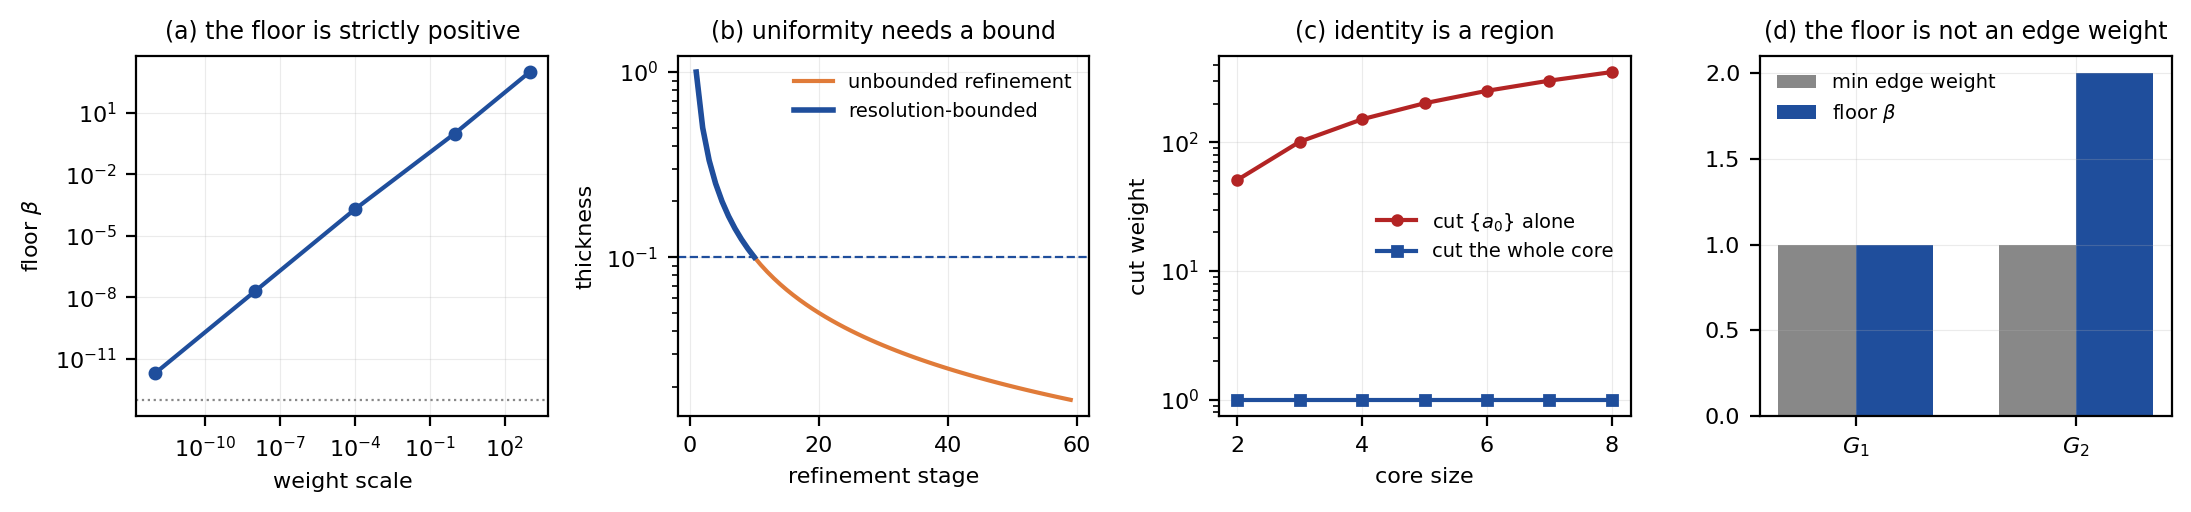
\includegraphics[width=\textwidth]{figures/fig1_substrate.png}
\caption{\textbf{The substrate.}
\textbf{(a)}~The floor is strictly positive across five orders of magnitude of
weight scale, including an instance whose smallest edge is $10^{-12}$.
\textbf{(b)}~Uniformity requires a bound. A system refining without limit
generates thicknesses $1/n$, each positive with infimum zero (orange);
truncating to ten stages restores a floor at $0.1$ (blue).
\textbf{(c)}~Identity is a region (\Cref{prop:region}): cutting $a_0$ alone
from a tightly packed core costs $W(n-1)+1$ and grows with core size, while
cutting the whole core costs $1$. Every minimiser therefore contains the core.
\textbf{(d)}~The floor is not an edge weight (\Cref{rem:notedge}). Two graphs
with identical minimum edge weight $1.0$ have floors $1$ and $2$; the
difference is invisible to any query over stored weights and is exactly what
\Cref{thm:separation} turns on.}
\label{fig:substrate}
\end{figure*}

% =====================================================================
\section{The ladder}
\label{sec:ladder}

We now define the object applied as a stencil.

\begin{definition}[Alignment]
\label{def:alignment}
For disjoint regions $x, x^\star$ the \emph{alignment} is
$a(x,x^\star)=\sepc(x,x^\star)/\Tot \in (0,1]$, where $\sepc(x,x^\star)$ is
the minimum weight of a cut separating them.
\end{definition}

\begin{lemma}[Alignment is floored]
\label{lem:alignfloor}
$a(x,x^\star) \geq \flo/\Tot > 0$.
\end{lemma}

\begin{proof}
Any separating cut is non-empty, and by \Cref{thm:floor} its weight is at
least $\flo$; divide by $\Tot>0$. The upper bound is
$\cut(S) \subseteq E$.
\end{proof}

\begin{definition}[Rung and power]
\label{def:rung}
A \emph{rung} toward target $x^\star$ is a map $R$ on regions whose
application commits a contact. Its \emph{power} at $x$ is the fraction of the
above-floor alignment it closes,
\begin{equation}
\pow(R,x) \;=\;
\frac{a(x,x^\star)-a(R(x),x^\star)}{a(x,x^\star)-\flo/\Tot} \;\in\; [0,1].
\label{eq:power}
\end{equation}
A rung is \emph{inert} if $\pow=0$ and \emph{absolute} if $\pow=1$.
\end{definition}

\begin{definition}[Ladder]
\label{def:ladder}
A \emph{ladder} is a finite sequence of rungs applied in order, each to the
output of the last, with \emph{power sequence} $(\pow_1,\dots,\pow_n)$.
\end{definition}

\begin{remark}[What a rung is not]
\label{rem:rungisnot}
\Cref{def:rung} mentions no property of $R$ beyond the alignment it closes:
not what it is made of, not how it operates, not how long it takes. Two rungs
with the same power are, at this resolution, the same rung. This is what makes
the ladder a stencil: it can be laid over records fetched from any source,
because it asks of them only a number. It is worth contrasting with the usual
criteria for whether two catalysts are ``the same kind'' --- mechanism, fold,
active-site residues, sequence homology --- which are known to disagree with
one another \citep{khersonsky2010}.
\end{remark}

\begin{theorem}[Multiplicative composition]
\label{thm:compose}
A ladder with power sequence $(\pow_1,\dots,\pow_n)$ has composite power
\begin{equation}
\pow(\Lad) \;=\; 1-\prod_{i=1}^{n}(1-\pow_i).
\label{eq:compose}
\end{equation}
\end{theorem}

\begin{proof}
Write $g_i = a(x_i,x^\star)-\flo/\Tot$ for the above-floor gap after $i$
rungs. By \Cref{eq:power}, $\pow_i=(g_{i-1}-g_i)/g_{i-1}$, so
$g_i=(1-\pow_i)g_{i-1}$, and by induction
$g_n = g_0\prod_{i\leq n}(1-\pow_i)$. The fraction of the initial gap closed
is $1-g_n/g_0$, which is \Cref{eq:compose}.
\end{proof}

\begin{corollary}[Repetition saturates]
\label{cor:saturate}
Repeating one rung of power $\pow$ gives composite $1-(1-\pow)^n$, which is
strictly increasing, tends to $1$, and attains it at no finite $n$. Copies of
what already works have geometrically diminishing returns: the $n$-th
repetition contributes $\pow(1-\pow)^{n-1}$.
\end{corollary}

\begin{proposition}[Cost of a target]
\label{prop:cost}
Reaching composite power $\pow^\star$ with rungs of power at most $\pow_{\max}$
requires at least
$\lceil \log(1-\pow^\star)/\log(1-\pow_{\max}) \rceil$ rungs.
\end{proposition}

\subsection{Sensitivity, and a correction}
\label{sec:sensitivity}

\begin{proposition}[Additive sensitivity]
\label{prop:additive}
With $P=\prod_i(1-\pow_i)$,
$\partial\pow(\Lad)/\partial\pow_j = P/(1-\pow_j)$, which is increasing in
$\pow_j$ and hence maximised at the \emph{highest}-power rung.
\end{proposition}

\begin{proof}
Differentiate \Cref{eq:compose}.
\end{proof}

This is a counter-intuitive result: it says the rung worth improving is the
strongest, not the bottleneck. We state the qualification it requires, because
without it the claim misleads.

\begin{proposition}[Proportional sensitivity is flat]
\label{prop:proportional}
Let improvement be proportional to a rung's remaining headroom, so rung $j$ is
raised by $\delta(1-\pow_j)$ rather than by $\delta$. Then the gain in
composite power is $\delta P$, independent of $j$.
\end{proposition}

\begin{proof}
Multiply the derivative of \Cref{prop:additive} by $\delta(1-\pow_j)$; the
factors $(1-\pow_j)$ cancel.
\end{proof}

\begin{remark}[Which parametrisation applies is an empirical question]
\label{rem:sens-honest}
The derivative of \Cref{prop:additive} prices an \emph{additive} increment
applied equally at every rung. Under proportional improvement --- raising a
rung by a fixed fraction of its own headroom, which is what ``improve this
catalyst by ten per cent'' ordinarily means --- the sensitivity is flat. Our
suite measures both: the additive argmax is the highest-power rung in
$5000/5000$ ladders, and the proportional spread across rungs is
$1.1\times10^{-16}$, machine zero, in $5000/5000$
(\Cref{sec:res-a}, \Cref{fig:ladder}(d)).

So the counter-intuitive direction is real under one parametrisation and
absent under another, and which applies depends on how improvements are
actually purchased in the laboratory. A check comparing the analytic
derivative against a numerical one cannot detect this, because both quantities
are the same additive derivative. We state the qualification rather than the
headline.
\end{remark}

\subsection{Closed ladders}
\label{sec:closed}

A linear ladder runs toward a target. A ring has none: it returns. Composite
power is undefined for it, and two invariants take its place.

\begin{definition}[Circulation and uniformity]
\label{def:invariants}
For a closed ladder with profile $(\pow_1,\dots,\pow_n)$, all $\pow_i<1$,
\begin{equation}
\circu = -\sum_{i=1}^n \log(1-\pow_i),
\qquad
\unif = \max\Bigl(0,\ 1-\tfrac{\mathrm{sd}(\pow)}{\mathrm{mean}(\pow)}\Bigr).
\label{eq:invariants}
\end{equation}
\end{definition}

\begin{proposition}[Properties]
\label{prop:invprops}
Both invariants are unchanged by rotation of the cycle; $\circu$ is additive
over concatenation of arcs and vanishes exactly when every rung is inert.
\end{proposition}

\begin{proof}
Both are functions of the multiset $\{\pow_i\}$, which rotation permutes
trivially. Additivity is additivity of a sum. Each term $-\log(1-\pow_i)\geq0$
with equality iff $\pow_i=0$.
\end{proof}

\begin{remark}[Where circulation is redundant, stated plainly]
\label{rem:rho-honest}
For a \emph{linear} ladder $\circu = -\log(1-\pow(\Lad))$ exactly, verified to
$10^{-13}$ over $500$ random ladders (\Cref{sec:res-a}). It is therefore a
monotone reparametrisation of composite power and adds no information whatever
in the linear case. We say this rather than let a new symbol suggest a new
quantity. Its content is entirely that it is defined \emph{without a target},
so it survives the passage to a cycle where composite power does not.

The invariant that genuinely adds information is $\unif$: over $4000$ pairs of
ladders constructed to share a composite power exactly, $2518$ differed in
$\unif$. A description recording only composite power cannot see the
difference.
\end{remark}

\begin{proposition}[Length is not recoverable]
\label{prop:length}
Closed ladders of different length may share both invariants, so $n$ must be
carried separately. A uniform cycle of length $n$ at power $\pow$ and one of
length $2n$ at $\pow'$ with $(1-\pow')^2 = 1-\pow$ have equal $\circu$ and
equal $\unif=1$.
\end{proposition}

\begin{figure*}[t]
\centering
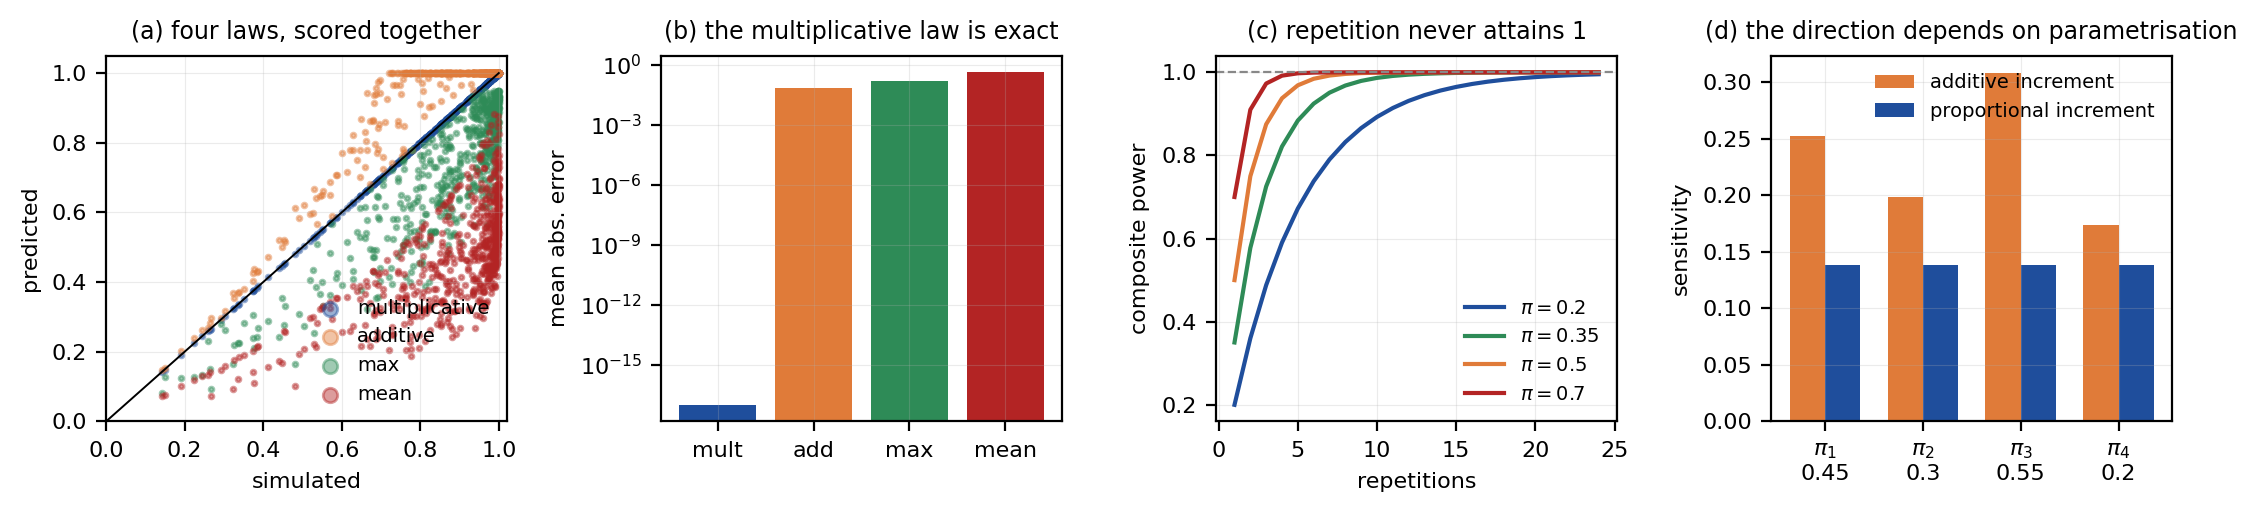
\includegraphics[width=\textwidth]{figures/fig2_ladder.png}
\caption{\textbf{The ladder algebra.}
\textbf{(a)}~Four candidate composition laws scored against rung-by-rung
simulation on $600$ random ladders. Scoring only the favoured law would not
have distinguished it; the comparison is the test.
\textbf{(b)}~Mean absolute error by law, logarithmic axis. The multiplicative
law is exact to machine precision; the alternatives err by $5.4\times10^{-2}$,
$1.5\times10^{-1}$ and $4.3\times10^{-1}$.
\textbf{(c)}~Repetition of a single rung rises strictly toward $1$ and reaches
it at no finite $n$ (\Cref{cor:saturate}).
\textbf{(d)}~The sensitivity correction (\Cref{rem:sens-honest}). Under an
additive increment (orange) sensitivity varies across rungs and is maximised
at the strongest, $\pow_3=0.55$; under a proportional increment (blue) it is
identical at every rung. The counter-intuitive direction is a property of the
parametrisation, not of the ladder.}
\label{fig:ladder}
\end{figure*}

% =====================================================================
\part{What Retrieval Cannot Do}
% =====================================================================

\section{Admissibility is not retrieval}
\label{sec:separation}

\subsection{Two kinds of question}

A query language over a stored graph evaluates patterns against triples. In
their core fragments SPARQL and its relatives are conjunctive queries with
regular path expressions \citep{perez2009,angles2017}: evaluation finds
homomorphisms from a pattern into the data, so everything returned is a
substructure of what was stored. That is the correct semantics for a
container.

\begin{definition}[Retrieval query]
\label{def:retrieval}
Let $G$ be a finite set of triples. A \emph{retrieval query} assigns to $G$ a
set of tuples computed by pattern matching and path composition on $G$ alone.
\end{definition}

\begin{definition}[Accountable propagation]
\label{def:accountable}
Fix $\varepsilon \geq 0$. A propagation from $x$ to $x^\star$ is
\emph{$\varepsilon$-accountable} if
$a(x,x^\star) \leq \flo/\Tot + \varepsilon$. Unfolding
\Cref{def:alignment}, this is
\begin{equation}
\sepc(x,x^\star) \;\leq\; \flo + \varepsilon\,\Tot .
\label{eq:accunfolded}
\end{equation}
\end{definition}

\begin{definition}[Admissibility query]
\label{def:admissibility}
Given $\Gph$, an item $v_0$, a target $x^\star$ and a tolerance, the
\emph{admissibility query} returns whether an accountable propagation exists,
together with its alignment.
\end{definition}

At $\varepsilon=0$ the total $\Tot$ cancels and the verdict is a comparison of
two numbers: a single minimum cut, and the floor. The first is local to the
queried pair. The second is a minimum over \emph{every} vertex in the system.
The separation below is the observation that these two can be moved
independently, and that a triple records neither.

\subsection{The separation}

\begin{theorem}[Retrieval cannot express admissibility]
\label{thm:separation}
There exist grounded contact graphs $\Gph_1, \Gph_2$ on the same vertex set,
with the same contact relation, and a pair $(v_0,x^\star)$, such that
\begin{enumerate}[label=(\roman*),leftmargin=2.2em]
\item $q(G_1)=q(G_2)$ for every retrieval query $q$, where $G_i$ records the
      contact relation of $\Gph_i$; while
\item an accountable propagation from $v_0$ to $x^\star$ exists in one and not
      in the other, at $\varepsilon=0$.
\end{enumerate}
\end{theorem}

\begin{proof}
Let $V=\{v_0,x,y_1,\dots,y_n,\med\}$ with $n \geq 1$. In both graphs the edges
are $\{v_0,x\}$ and $\{u,\med\}$ for every $u \neq \med$. Both are grounded.

Assign weights. In both, $w(\{v_0,x\})=1$ and the medium edges at $v_0$ and
$x$ have weight $1$. The graphs differ only in the medium edges at the $y_i$:
weight $1$ in $\Gph_1$, weight $2$ in $\Gph_2$.

\emph{(i)} The edge sets are equal, so the recorded contact relations coincide
as sets of triples. Any $q$ in the sense of \Cref{def:retrieval} is a function
of its argument alone, hence agrees on them. A triple asserts that a relation
holds and carries no cost, so there is nothing here for retrieval to see.

\emph{(ii)} The $y_i$ are joined only to $\med$, so they lie on no
$v_0$--$x$ path and no minimum such cut uses their edges: the cheapest
separation places $v_0$ alone, severing $\{v_0,x\}$ and the medium edge at
$v_0$, so $\sepc(v_0,x)=2$ in \emph{both} graphs. The floor is a minimum over
all vertices. Isolating $v_0$ or $x$ costs $2$; isolating $y_i$ severs its
single medium edge, costing $1$ in $\Gph_1$ and $2$ in $\Gph_2$. Hence
$\flo_1 = 1$ and $\flo_2 = 2$. Applying \Cref{eq:accunfolded} at
$\varepsilon=0$: in $\Gph_2$, $\sepc = 2 \leq 2 = \flo_2$ and the propagation
is accountable; in $\Gph_1$, $\sepc = 2 > 1 = \flo_1$ and it is not.
\end{proof}

\begin{remark}[What the separation is about]
\label{rem:sepmeaning}
The construction turns on one asymmetry. The queried quantity
$\sepc(v_0,x^\star)$ depends on weights along $v_0$--$x^\star$ separations;
the threshold $\flo$ depends on a minimum over every item in the system,
including items lying on no path between the two and, from the query's point
of view, entirely irrelevant. Editing a weight at the $y_i$ changes the
verdict about $(v_0,x^\star)$ without changing anything a pattern-matcher
could match.

So \emph{accountability is a global property expressed in local terms}, and a
stored graph records only the local terms.
\end{remark}

\begin{corollary}[Attributed triples do not close the gap]
\label{cor:attributed}
Extending \Cref{def:retrieval} to allow numeric attributes on triples and
arithmetic comparison in patterns does not make admissibility expressible.
\end{corollary}

\begin{proof}
By \Cref{thm:separation} the verdict depends on $\flo$, a minimum over items
of a minimum over subsets. Conjunctive queries with regular path expressions
are evaluated by matching bounded patterns
\citep{perez2009,angles2017,barcelo2013}; the
fragment contains no operator forming a minimum over subsets of the domain,
and comparing stored attributes does not introduce one. The obstruction is
expressibility, not hardness: a minimum cut is computable in polynomial time
\citep{fordfulkerson1956,stoer1997}, so the quantity is cheap to compute and
impossible to phrase; multi-terminal variants are equally classical
\citep{gomory1961,menger1927}.
\end{proof}

Our suite executes \Cref{cor:attributed} directly: with weights stored as
triple attributes, the minimum edge weight is $1.0$ in both graphs while the
floors are $1$ and $2$ (\Cref{sec:res-b}).

\subsection{Two representations, one system}

It would be a misreading of \Cref{thm:separation} to conclude that stored
graphs are useless. The correct conclusion is sharper.

\begin{theorem}[Representational partition]
\label{thm:partition}
A description-logic defined class over participant roles cannot express a
residue chain, and a residue chain does not determine the stoichiometric
coefficients of its participants. Hence the signature view and the chain view
answer disjoint sets of questions, and neither is a refinement of the other.
\end{theorem}

\begin{proof}
\emph{Signatures cannot carry mechanism.} A residue chain is a finite sequence
with state: the cut at step $i$ is the boundary condition of step $i+1$.
Expressing it requires quantification over positions and a successor relation
with transitive closure. $\mathcal{SROIQ}$, the description logic underlying
OWL 2, admits transitive roles but not the composition of a transitive role
with the value restrictions needed to thread state along it without losing
decidability \citep{baader2003,horrocks2006,grau2008}. A defined class can therefore
state that a reaction \emph{has} a participant with a role, but not that its
steps occur in an order; an ordering is exactly what a kinetic mechanism
specifies \citep{cleland1963}.

\emph{Chains cannot carry stoichiometry.} A chain records which items were
individuated and at what cost. A process consuming two equivalents of a
reactant and one consuming one produce chains differing in the number of cuts,
but the framework provides no map from cut count back to coefficient: an item
individuated once and used twice is indistinguishable, at the level of
committed boundary, from an item individuated twice.
\end{proof}

\begin{remark}[The practical reading]
\label{rem:partition-practical}
This is why a practitioner building one ontology for a reaction domain finds
that the questions will not sit together, and ends by recommending separate
linked modules for reactions, substances, measurements and workflows. The
module boundaries are the blocks of \Cref{thm:partition}: standards for
pathway exchange \citep{demir2010} and term hierarchies \citep{ashburner2000}
sit on one side of it. We offer this as an interpretation rather than a
theorem: we show the partition exists, and that its blocks correspond to a
boundary practitioners draw independently.
\end{remark}

% =====================================================================
\section{The medium}
\label{sec:medium}

The contact graph of \Cref{def:contactgraph} has a medium vertex to which
everything is adjacent and which no result has yet used. Giving it content
turns two annotations into computations.

\begin{definition}[Medium as reservoir]
\label{def:medium}
The \emph{medium} is a pair $\med=(\mu,\tau)$ where $\mu$ assigns to each
chemical identity $i$ an \emph{ambient occupancy} $\mu(i) \geq 0$, and
$\tau>0$ is the \emph{exchange scale}: the occupancy change the medium absorbs
without itself being individuated. The weight of the edge from a leaf $\ell$
of identity $i$ to $\med$ is
\begin{equation}
w(\ell,\med) \;=\; \flo\bigl(1+\log(1+\tau/\mu(i))\bigr),
\qquad \mu(i)>0,
\label{eq:mediumweight}
\end{equation}
and $w(\ell,\med)=\infty$ when $\mu(i)=0$.
\end{definition}

\begin{remark}[The constitutive choice, and what depends on it]
\label{rem:constitutive}
\Cref{eq:mediumweight} is a modelling choice and we justify it by three
properties rather than deriving it. It never violates the floor, since the
bracket is at least $1$. Abundance is cheap to individuate against and
scarcity is expensive: as $\mu \to \infty$ the weight falls to $\flo$ (a leaf
surrounded by copies of itself is barely distinguishable from its
surroundings) and as $\mu \to 0^+$ it diverges. And only the ratio $\tau/\mu$
appears, so $\tau$ and $\mu$ are never separately observable.

Every result below uses \Cref{eq:mediumweight} only through the facts that it
is strictly decreasing in $\mu$ and bounded below by $\flo$. Our suite
re-verifies each structural result under four unrelated weight families
sharing only those two properties --- logarithmic, square-root, rational and a
non-smooth linear cap --- so that no theorem depends on the logarithm
(\Cref{fig:medium}(a)).
\end{remark}

\subsection{Solvent role is computed}

A five-class leaf algebra with a single \textsf{solvent} class conflates two
chemically distinct things: a small number of ordered waters that occupy
defined positions, make specific hydrogen bonds and mediate recognition
\citep{levy2006,creighton1993}, and the bulk remainder, which is a medium
rather than a participant \citep{ball2008}.

\begin{definition}[Structural residue and role]
\label{def:role}
Let $\ell$ be a solvent leaf of identity $i$, and $N(\ell)$ the leaves other
than $\med$ adjacent to it. The \emph{structural residue} is
$\rho_{\mathrm{str}}(\ell)=\sum_{u \in N(\ell)} w(\ell,u)$, the boundary
$\ell$ maintains against the system, as distinct from $w(\ell,\med)$, the
boundary it maintains against its surroundings. Then
\begin{equation}
\mathrm{role}(\ell) \;=\;
\begin{cases}
\textsf{structural} & \text{if } \rho_{\mathrm{str}}(\ell) \geq w(\ell,\med),\\
\textsf{bulk} & \text{otherwise.}
\end{cases}
\label{eq:role}
\end{equation}
\end{definition}

\begin{theorem}[Role is decidable at the floor]
\label{thm:role}
For every solvent leaf, $\mathrm{role}(\ell)$ is determined by the contact
graph and the medium alone, requires no annotation, and is invariant under any
rescaling of $w$ preserving the floor. Moreover a leaf with no system contacts
is \textsf{bulk}, and role is monotone in $\mu(i)$: increasing ambient
occupancy can turn a bulk leaf structural but never the reverse.
\end{theorem}

\begin{proof}
Determinacy and invariance are immediate: both sides of \Cref{eq:role} are
sums of edge weights, and the comparison is a ratio test, hence invariant
under $w \mapsto cw$ for $c>0$ provided $c\flo$ is taken as the new floor. If
$N(\ell)=\varnothing$ then $\rho_{\mathrm{str}}=0$ while
$w(\ell,\med)\geq\flo>0$, so the test fails and the role is \textsf{bulk}. For
monotonicity, $w(\ell,\med)$ is strictly decreasing in $\mu(i)$ by
\Cref{rem:constitutive} while $\rho_{\mathrm{str}}$ does not depend on it, so
increasing $\mu(i)$ lowers the right-hand side and cannot falsify a passing
test.
\end{proof}

\begin{corollary}[The role question is answered by computation]
\label{cor:rolecomputed}
``What is the role of the solvent in this reaction?'' has an answer of the
form ``\textsf{structural}, because $\rho_{\mathrm{str}}=x \geq
w(\cdot,\med)=y$'', derived from the graph. No curator supplies it and no
vocabulary term records it.
\end{corollary}

Our suite exhibits two waters of identical chemical identity receiving
opposite roles: an ordered active-site water with
$\rho_{\mathrm{str}}=4\flo$ is \textsf{structural}, and a bulk water with no
system contacts is \textsf{bulk} (\Cref{sec:res-c},
\Cref{fig:medium}(b)).

\subsection{Direction is a property of the medium}

A knowledge graph over reactions must record directionality and cannot do it
with a boolean. The public reaction resource we queried stores
$18\,907$ bidirectional master reactions and $37\,814$ directional children,
exactly two per master: for the alanine transaminase reaction
$\mathrm{RHEA}{:}19453$, ``L-alanine + 2-oxoglutarate = pyruvate +
L-glutamate'', the children are $19454$ and $19455$. The same master
identifier names a reaction that runs one way in one organism and the other
way in another. The distinction ``reversible in principle, irreversible
physiologically'' is real, load-bearing, and in every representation we know
of it is \emph{asserted} by a curator.

\begin{lemma}[Reversal invariance of the chain]
\label{lem:reversal}
Let $C=(S_1,\dots,S_k)$ be a chain with residues $\rho_i=w(\cut(S_i))$ and
$C^R$ its reversal. Then $C$ and $C^R$ commit the same total boundary, the
same number of cut events, and the same set of committed edges.
\end{lemma}

\begin{proof}
Each $\rho_i$ is the weight of an edge boundary, a quantity of the graph and
not of the order in which boundaries are committed. Summation is commutative,
the cut count is the cardinality $k$, and the committed edge set is
$\bigcup_i \cut(S_i)$: all three are invariant under permutation and in
particular under reversal.
\end{proof}

\begin{corollary}[Cut structure cannot orient]
\label{cor:cannotorient}
No predicate definable from the residues, the cut count, or the committed
boundary distinguishes $C$ from $C^R$. Direction must come from outside the
chain.
\end{corollary}

\begin{definition}[Medium bias]
\label{def:bias}
For a chain from initial multiset $I$ to terminal multiset $T$ evaluated in
medium $\med$, the \emph{medium bias} is
\begin{equation}
\Delta_\med(C) \;=\; \sum_{i \in T} w(\ell_i,\med)
                  \;-\; \sum_{i \in I} w(\ell_i,\med).
\label{eq:bias}
\end{equation}
\end{definition}

By \Cref{eq:mediumweight}, $\Delta_\med(C)>0$ exactly when the products are on
balance \emph{scarcer} in the medium than the reactants, and
$\Delta_\med(C^R)=-\Delta_\med(C)$ by construction.

\begin{theorem}[Direction trichotomy]
\label{thm:trichotomy}
Let $\delta=\Delta_\med(C)$. Exactly one of the following holds.
\begin{enumerate}[label=(\alph*),leftmargin=2.2em]
\item $\delta > \flo$: the process is irreversible in the direction of $C$.
\item $\delta < -\flo$: the process is irreversible in the direction of $C^R$.
\item $\abs{\delta} \leq \flo$: the process is reversible in principle and
      undirected in this medium.
\end{enumerate}
Consequently reversibility is a property of the pair (chain, medium) and not
of the chain, and the same chain may fall in different cases in different
media.
\end{theorem}

\begin{proof}
The three cases are exhaustive and mutually exclusive as a trichotomy on the
real number $\delta$ against $\flo>0$. The floor appears because a bias
smaller than $\flo$ is a distinction the receiver cannot make: a medium
favouring one direction by less than the floor does not favour it at all. The
final clause is immediate because $\delta$ depends on $\med$ through
\Cref{eq:bias} while the chain's own admissibility does not.
\end{proof}

\begin{corollary}[One identifier, two directions]
\label{cor:oneidentifier}
Two organisms whose media differ in the ambient occupancy of a shared
participant may run the same chain in opposite directions, and both are
correct. The reaction identifier names the chain, which is
direction-symmetric by \Cref{lem:reversal}; the direction is named by the
medium, which the identifier does not carry.
\end{corollary}

Our suite computes the trichotomy for $\mathrm{RHEA}{:}19453$ in three media
and reaches all three cases: $\delta/\flo = +5.20$ in a
glutamate-depleted cytosol (forward), $-3.82$ in a 2-oxoglutarate-depleted one
(reverse), and exactly $0$ in a balanced medium (undirected). The third is a
negative control: without a medium that \emph{refuses} to orient, the
trichotomy would be a dichotomy with a decorative third branch
(\Cref{fig:medium}(d)).

\subsection{A saturation asymmetry we did not anticipate}

\begin{proposition}[Flooding cannot reverse a chain]
\label{prop:saturation}
Let $C$ be a balanced chain whose identities all sit at a common baseline
occupancy $\mu_0$, and let one terminal identity be made arbitrarily abundant.
Then under \Cref{eq:mediumweight}
\begin{equation}
\Delta_\med(C) \;\longrightarrow\; -\flo\log\!\bigl(1+\tau/\mu_0\bigr)
\qquad \text{as } \mu \to \infty,
\label{eq:saturation}
\end{equation}
so the attainable bias is bounded. Depletion of a reactant carries no such
bound.
\end{proposition}

\begin{proof}
Each baseline identity contributes $w=\flo(1+\log(1+\tau/\mu_0))$. Making one
terminal identity abundant sends its contribution to $\flo(1+\log 1)=\flo$, so
the terminal sum falls by exactly $\flo\log(1+\tau/\mu_0)$ while the initial
sum is unchanged, giving \Cref{eq:saturation}. For the second clause,
$\mu \to 0^+$ sends $w(\ell,\med) \to \infty$ by \Cref{eq:mediumweight}, so
the bias is unbounded.
\end{proof}

\begin{remark}[How this was found]
\label{rem:saturation-found}
We did not anticipate \Cref{prop:saturation} and would not have found it by
inspection. An earlier sweep of the trichotomy varied only the product-end
occupancy and reached case (a) and case (c) but never case (b), which looked
like a refutation of \Cref{thm:trichotomy}. The theorem was not at fault: the
sweep was one-sided, and a one-sided sweep cannot reach case (b) for the
reason now recorded as \Cref{prop:saturation}. At $\mu_0=10^{-4}$ and
$\tau=10^{-3}$ the measured limit is $-2.397895\,\flo$ against the predicted
$-\log(11)\,\flo = -2.397895\,\flo$, agreeing to six decimal places, and
thirty orders of magnitude of further flooding move it no further; depletion
over the same range reaches $-22.93\,\flo$ and continues
(\Cref{fig:medium}(c)).

Read chemically: \emph{product inhibition cannot reverse a reaction; only
substrate depletion can}. We report the episode because a suite written to
pass would have hidden it.
\end{remark}

\begin{figure*}[t]
\centering
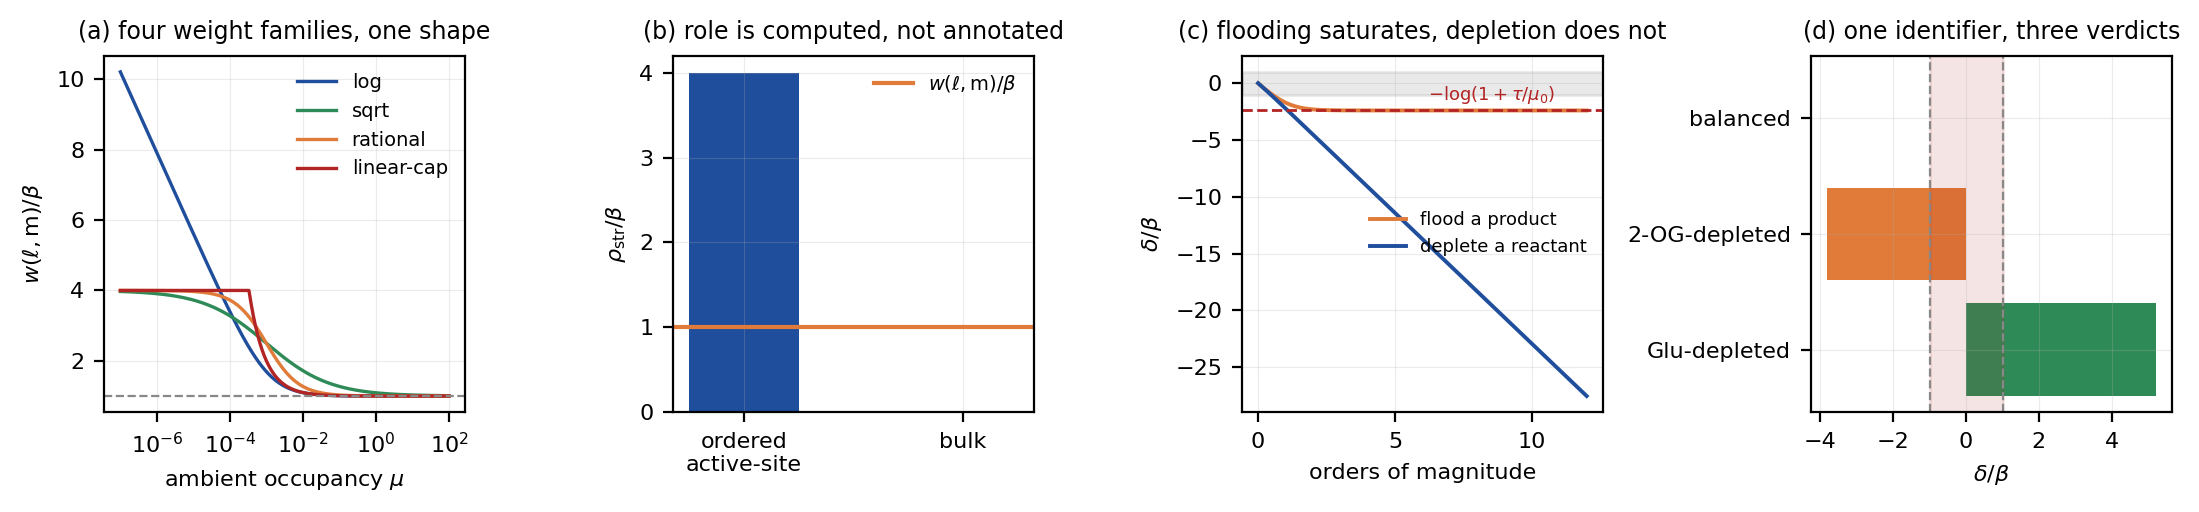
\includegraphics[width=\textwidth]{figures/fig3_medium.png}
\caption{\textbf{The medium.}
\textbf{(a)}~Four weight families satisfying \Cref{rem:constitutive}. All are
bounded below by $\flo$ (dashed) and strictly decreasing in ambient occupancy.
Every structural theorem is re-verified under all four, so no result depends
on the logarithm.
\textbf{(b)}~Solvent role is computed, not annotated (\Cref{thm:role}). Two
waters of identical chemical identity: the ordered active-site water holds
$\rho_{\mathrm{str}}=4\flo$ against the system and is \textsf{structural}; the
bulk water holds none and is \textsf{bulk}. The orange line is the competing
boundary $w(\ell,\med)$.
\textbf{(c)}~The saturation asymmetry (\Cref{prop:saturation}). Flooding a
product (orange) approaches the ceiling $-\log(1+\tau/\mu_0)$ (red dashed) and
stops; depleting a reactant (blue) descends without bound. Reversing a chain
requires depletion, not flooding --- an asymmetry found by a failing test.
\textbf{(d)}~One reaction identifier, three verdicts
(\Cref{cor:oneidentifier}). The same chain is forward in one medium, reverse
in another, and undirected in a balanced one; the grey band is the refusal
region $\abs{\delta} \leq \flo$.}
\label{fig:medium}
\end{figure*}

% =====================================================================
\part{The Architecture}
% =====================================================================

\section{The plan language and its verdicts}
\label{sec:plan}

\subsection{Why a plan language and not a query language}

Federating heterogeneous sources is an old problem with a long literature
\citep{halevy2006pdms,buil2013federated}; the observation below is narrower.
The sources a catalysis question must cross --- a reaction knowledge base with
a SPARQL endpoint \citep{bansal2022}, a protein resource exposing both SPARQL
and REST \citep{uniprot2023}, a pathway resource exposing only flat files
\citep{kanehisa2000,milacic2024}, an electronic laboratory notebook ---
do not share a query model, and no amount of engineering will give them one.
They do share a \emph{result} model: finite sets of identifiers carrying
attributes.

\begin{principle}[Terms denote results]
\label{prin:results}
A language whose terms denote result sets and whose operators denote
instructions on what to do with a result is portable across backends in a way
that a language whose terms denote graph patterns cannot be. Queries are its
leaves and are never written by the user.
\end{principle}

This is what removes the \emph{querying requirement} of \Cref{sec:intro}: the
asker states what they want done with a result, not how the curator spelled
it.

\begin{definition}[Source]
\label{def:source}
A \emph{source} is a triple of an endpoint, a declared \emph{capability set}
--- the structural features it can state --- and an extraction function.
\end{definition}

\begin{theorem}[Static capability containment]
\label{thm:static}
Lowering a plan step to a source is total exactly on the steps whose required
capabilities are contained in the source's declared set. Containment is
decidable before any request is issued.
\end{theorem}

\begin{proof}
A step declares a finite set $r$ of required features; a source declares a
finite set $c$. Lowering emits a query for each feature of $r$; it succeeds
exactly when each has a lowering rule, which holds exactly when $r \subseteq
c$. Both sets are finite and given in advance, so $r \subseteq c$ is decidable
statically.
\end{proof}

\begin{remark}[Capability is a claim about a compiler]
\label{rem:capability}
``This system supports counting'' is true or false of a lowering procedure,
not of the target logic. The two come apart in both directions: a formalism
may express what no compiler lowers, and a compiler may lower what the
formalism does not entail. Only the compiler-level reading admits the
decidable check of \Cref{thm:static}.
\end{remark}

\subsection{Six verdicts}

\begin{definition}[Verdict]
\label{def:verdict}
A step returns one of
\begin{center}
\begin{tabular}{@{}ll@{}}
\vans & a result set, certified non-empty\\
\vempty & the question is well posed and the answer is certified empty\\
\vexp & the question cannot be stated in the source's model\\
\vsurf & statable in the model, not lowerable by this compiler\\
\vstarve & this step failed because an earlier step under-retrieved\\
\vhaust & the budget ran out before the step completed\\
\end{tabular}
\end{center}
\end{definition}

\begin{theorem}[Non-degeneracy]
\label{thm:nondegeneracy}
No verdict other than \vans{} may carry a non-empty payload, and \vans{} may
not carry an empty one unless emptiness is itself certified.
\end{theorem}

\begin{proof}
Suppose a verdict $V \neq \vans$ carried a non-empty payload. A caller
consuming payloads would then act on results from a step reporting that it did
not answer, so $V$ and \vans{} would be indistinguishable to that caller,
collapsing the verdict space to the boolean it exists to refine. The second
clause is symmetric: an uncertified empty \vans{} is exactly the conflation of
\Cref{sec:fivecases}.
\end{proof}

This is a structural property, not a reporting discipline. In our reference
kernel it is enforced by the constructor: attempting to build a \vstarve{}
result carrying a payload raises, and our suite checks that it does
(\Cref{sec:res-c}).

\begin{remark}[On budgets]
\label{rem:budget}
A plan spends a finite retrieval budget across sources whose yields differ.
Where each source's yield is concave in the effort spent on it, the optimal
split equalises marginal return --- the water-filling rule familiar from
resource allocation under a concave objective \citep{boyd2004}. We do not
develop the allocator here, and note only that a budget exceeding the sum of
minimum step costs is necessary but not sufficient for a plan to complete,
since a step may starve on a predecessor rather than on its own funding.
Enumeration over a handful of federated sources is affordable
\citep{cormen2009}.
\end{remark}

\begin{proposition}[Starvation is the characteristic federated failure]
\label{prop:starve}
\vstarve{} is reachable only when a step's input is produced by another step,
which is the federated setting. A starved step must name the predecessor at
fault, and a walk up those names terminates.
\end{proposition}

\begin{proof}
In a single-source query a step's input is the corpus, which does not
under-retrieve; the verdict is unreachable. In a plan, step $j$ may receive
empty bindings from step $i<j$ although $i$ answered correctly under its own
declaration. Blame is assigned to $i$; since indices strictly decrease, the
walk terminates.
\end{proof}

\subsection{The stencil}

We can now state what the architecture does with a fetched record.

\begin{construction}[Ladder as stencil]
\label{con:stencil}
Given records fetched by a plan, translate them into a contact graph
(\Cref{def:contactgraph}), declare a medium (\Cref{def:medium}), and lay a
ladder over the result: each contact in the process contributes a rung whose
power is computed from \Cref{eq:power} using the separation costs of the
translated graph. The composite power, the invariants of
\Cref{def:invariants}, the role of \Cref{eq:role} and the direction of
\Cref{thm:trichotomy} are then read off.
\end{construction}

\begin{remark}[Why this removes the modelling requirement]
\label{rem:nomodel}
The stencil asks of a record only what is needed to compute a separation cost.
It does not ask what class the record belongs to, which ontology term names its
relation, or whether a curator anticipated the question. A question such as
``in which direction is this reaction admissible here'' is therefore answerable
over records whose schema contains no notion of direction --- which is the
sense in which one may query items one cannot model.
\end{remark}

\begin{remark}[What the stencil costs, stated plainly]
\label{rem:stencil-honest}
Two costs are real and we name them. First, the translation from a record to a
contact graph supplies structure the record does not state --- implicit
hydrogens, inferred bond orders, a medium the record never mentions --- and a
downstream reader cannot distinguish a stated element from a supplied one
unless the translator tags them. Second, the powers used in
\Cref{sec:questions} are \emph{declared} rather than derived from measured
kinetics. Deriving them from retrieved data is the natural next step and we
have not taken it; \Cref{sec:limits} records both.
\end{remark}

\begin{figure}[t]
\centering
\begin{lstlisting}
plan bacterial_transaminase_no_cys

  source RXN  capability { reaction, participant, ec, equation }
  source PROT capability { protein, organism, lineage, sequence }

  let rxns  = fetch RXN  where participant contains "benzylethylamine"
  let enzs  = fetch PROT where catalyses in rxns
  let bact  = keep enzs  where lineage contains "Bacteria"
  let final = keep bact  where not contains(sequence, "C")

  require final nonempty
  emit final
\end{lstlisting}
\caption{A plan for question Q1. The user states what is wanted of a result;
no SPARQL is written. The last step is a predicate over a retrieved attribute
and is not a triple lookup: no public store holds a \texttt{hasCysteine} flag,
so a pattern-matching query returns nothing (\Cref{sec:res-b}). The plan is
checked against the declared capabilities before any request is issued
(\Cref{thm:static}).}
\label{fig:plan}
\end{figure}

% =====================================================================
\part{Validation}
% =====================================================================

\section{Protocol}
\label{sec:protocol}

The suite is designed on one principle: \emph{every check must be able to
fail}. Four experiments run in dependency order. Experiments A--C reach no
network and resolve against fixtures, so every number is reproducible offline.
Experiment D reaches a public endpoint and reports the live arm as untested
rather than failed if the service is unreachable.

Three devices make the suite capable of failing.

\begin{enumerate}[leftmargin=1.6em,itemsep=2pt]
\item \textbf{Negative controls.} Four checks assert that something does
      \emph{not} happen on well-formed input: that a constant statistic does
      not discriminate; that the query battery of \Cref{sec:res-b} separates a
      genuinely different contact relation; that a balanced medium refuses to
      orient; and that the miniature of \Cref{sec:res-d} returns nothing when
      asked for a root present in no record.
\item \textbf{Independent cross-checks.} The SPARQL results are computed on
      two independently developed engines, and the analytic sensitivity is
      checked against a numerical derivative that does not use the closed
      form.
\item \textbf{Non-discriminating checks are excluded from the score.} One
      check --- permuting a fixed multiset of powers --- cannot fail, because
      \Cref{eq:compose} is symmetric in its arguments. The hazard of a check
      that is present but does no work is the analogue of vacuous
      satisfaction in model checking \citep{beer2001,kupferman2003}. We report it as
      non-discriminating and exclude it rather than counting a pass.
\end{enumerate}

Software: Python 3.14, \texttt{rdflib} 7.6.0 \citep{rdflib},
\texttt{pyoxigraph} 0.5.9 \citep{pyoxigraph}, NumPy 2.4.3
\citep{harris2020numpy}. All measurements are dated 3 September 2026.

\section{Results}
\label{sec:results}

\subsection{Experiment A: the ladder algebra}
\label{sec:res-a}

Twenty-three scored checks; all pass. One further check is excluded as
non-discriminating, and one is a negative control.

The floor is computed rather than assumed on three instances, including an
adversarial one whose smallest edge weight is $10^{-12}$; every instance
returns a strictly positive floor. On that instance the floor is
$1.0+10^{-12}$ and \emph{not} $10^{-12}$, confirming \Cref{rem:notedge}: a
cheap edge inside an expensive cut does not make the cut cheap. The
complementary branch is exhibited separately --- a system refining without
limit produces thicknesses $1/n$ whose infimum is zero, and truncating to ten
stages restores a floor at $0.1$ --- so the hypothesis of \Cref{thm:uniform}
does real work.

\Cref{prop:region} is measured: in a graph with a four-vertex core of internal
weight $50$ joined to the periphery by a single edge, the minimiser for a core
vertex contains all four core vertices at cost $1$, and no singleton attains
it.

All four composition laws are scored against rung-by-rung simulation over
$4000$ ladders. The multiplicative law is exact to machine precision
($0.0$); the additive, maximum and mean laws err by
$5.45\times10^{-2}$, $1.49\times10^{-1}$ and $4.31\times10^{-1}$. Scoring only
the favoured law would not have distinguished it.

The sensitivity correction of \Cref{rem:sens-honest} is measured on $5000$
ladders: the additive argmax is the highest-power rung in $5000/5000$ cases,
and the proportional spread across rungs is $1.11\times10^{-16}$ in
$5000/5000$. The analytic derivative agrees with a numerical one to
$1.3\times10^{-10}$.

For closed ladders, $\circu$ reparametrises composite power on linear ladders
to $1.4\times10^{-13}$ over $500$ trials --- the redundancy of
\Cref{rem:rho-honest} made quantitative --- while $\unif$ separates $2518$ of
$4000$ ladder pairs constructed to share a composite power exactly.

\subsection{Experiment B: expressibility}
\label{sec:res-b}

Nine scored checks pass, one of them a negative control.

Two contact graphs are constructed as in \Cref{thm:separation}. They record
identical triples: six each, set difference empty. Their separation costs
agree, $\sepc(v_0,x)=2$ in both, and their floors differ, $\flo_1=1$ and
$\flo_2=2$, so the accountability verdicts are opposite --- inadmissible in
the first and admissible in the second.

Thirteen retrieval query forms were then run against both graphs on both
engines: all triples, triple count, per-node degree, neighbours, two ASK forms
over property paths, transitive closure, two-step neighbourhoods, adjacency to
the medium, distinct subject count, a two-hop join, an \texttt{OPTIONAL} with
\texttt{FILTER}, and a nested aggregate over grouped degree.
\textbf{No query separated the two graphs}, and the two engines agreed on
every query, $13/13$.

The negative control is the load-bearing row. The same battery run against a
third graph with a genuinely different contact relation separates it on
$8$ of $13$ queries. Without this, the result above would be consistent with a
blind battery.

\Cref{cor:attributed} is executed: with the weights stored as triple
attributes, a query for the minimum stored weight returns $1.0$ for
\emph{both} graphs, while their floors are $1$ and $2$. Storing the numbers
does not make the minimum-over-subsets expressible.

Finally the Q1 shape is executed. A query for a \texttt{hasCysteine} flag
returns nothing, because no such predicate was curated; the same question
asked as a computation over the retrieved sequence returns the correct two
proteins.

\subsection{Experiment C: twenty-eight questions}
\label{sec:res-c}\label{sec:questions}

Twenty scored checks pass, one of them a negative control.

Twelve questions were supplied by practitioners --- five from biocatalysis and
seven generic dataset queries in the shape of a chemistry data catalogue
profile --- without reference to this framework. We added sixteen to exercise
verdicts the twelve do not reach. \Cref{tab:questions} gives the resolution of
all twenty-eight. Twenty-one are answered and seven refused, and five distinct
verdicts occur.

Four findings are worth stating beyond the pass count.

\paragraph{The dataset filters discriminate.} Questions Q6--Q8 form a strictly
narrowing chain: three datasets mention the compound, two of those are of the
requested activity type, and one of those was measured on the named vendor's
instrument \emph{at the named setting}. Each added constraint removes at least
one dataset, so the filters are shown to discriminate rather than merely to
return a row. Restricting from ``a Bruker'' to ``a Bruker set to
$^{13}\mathrm{C}$'' removes a dataset: a configuration value is part of a
measurement's provenance.

\paragraph{One identifier, three verdicts.} The direction trichotomy reaches
all three cases on the alanine transaminase chain, as reported in
\Cref{sec:medium}. The balanced medium is a negative control and returns
$\delta=0$ exactly, refusing to orient.

\paragraph{Two waters, opposite roles.} \Cref{thm:role} is measured with
$w(\ell,\med)=3.700\times10^{-4}$: the ordered active-site water has
$\rho_{\mathrm{str}}=1.480\times10^{-3} \geq w$ and is \textsf{structural};
the bulk water has $\rho_{\mathrm{str}}=0 < w$ and is \textsf{bulk}.

\paragraph{The refusals carry remedies.} All seven refusals name both a
blocker and an unblock path, and the four verdict kinds reached are
distinguished by different mechanisms: \vexp{} by static capability
containment, \vsurf{} by a question that is not of retrieval type,
\vstarve{} by a predecessor that under-retrieved, and \vhaust{} by a budget.
In the budget case two steps answer and two report \vhaust{}; a rows-only
interface would have returned the same empty table for both.

\begin{table}[p]
\centering\small
\caption{All twenty-eight questions and their verdicts. Q1--Q12 were supplied
by practitioners; Q4$'$ and Q13--Q28 were added to exercise outcomes the
twelve do not reach. Every refusal carries a blocker and an unblock path;
those are abbreviated here and given in full in the results file.}
\label{tab:questions}
\begin{tabular}{@{}llll@{}}
\toprule
\textbf{\#} & \textbf{Question} & \textbf{Verdict} & \textbf{Blocker / note}\\
\midrule
\multicolumn{4}{@{}l}{\emph{Group 1 --- biocatalysis (practitioner-supplied)}}\\
Q1  & bacterial transaminase, no Cys      & \vans   & 2 sources + computed predicate\\
Q2  & buffer and pH for mt-X              & \vans   & laboratory record only\\
Q3  & substrate scope of BVMO-Y           & \vans   & aggregation over a screen\\
Q4  & expected products, kinetic resolution & \vsurf & not a retrieval question\\
Q5  & device and wavelength, 23 Mar       & \vans   & instrument provenance\\
\midrule
\multicolumn{4}{@{}l}{\emph{Group 2 --- generic dataset queries}}\\
Q6  & datasets about compound C           & \vans   & 3 datasets\\
Q7  & \dots of activity type T            & \vans   & narrows to 2\\
Q8  & \dots on a Bruker set to X          & \vans   & narrows to 1\\
Q9  & datasets about a reaction with product P & \vans & 4 datasets\\
Q10 & \dots with starting material C      & \vans   & 4 datasets\\
Q11 & \dots measured on UV-vis with C     & \vans   & 1 dataset\\
Q12 & \dots with catalyst S on a Bruker   & \vans   & 3 datasets\\
\midrule
\multicolumn{4}{@{}l}{\emph{Group 3 --- answerable without a model of the answer}}\\
Q4$'$ & direction of RXN 19453 per medium & \vans   & three verdicts, one identifier\\
Q13 & role of the solvent                 & \vans   & computed, not annotated\\
Q14 & which catalysts are interchangeable & \vans   & one number each, no structure\\
Q15 & which step may be deleted           & \vans   & predicted before experiment\\
\midrule
\multicolumn{4}{@{}l}{\emph{Group 4 --- refused, with named blockers}}\\
Q16 & derived reaction temperature        & \vexp   & floor insensitive at this depth\\
Q17 & buffer, from the reaction store     & \vexp   & capability containment fails\\
Q18 & enzymes for an unretrieved reaction & \vstarve & predecessor named\\
Q19 & four-step plan on a budget of two   & \vhaust & two steps unrun\\
\midrule
\multicolumn{4}{@{}l}{\emph{Group 5 --- extended battery}}\\
Q21 & reactions running both ways         & \vans   & two media\\
Q22 & bacterial enzymes for an EC         & \vans   & 2 enzymes\\
Q23 & pathways producing a lactone        & \vans   & 1 pathway\\
Q24 & experiments above pH 8              & \vans   & 1 experiment\\
Q25 & operators using UV-vis              & \vans   & 1 operator\\
Q26 & datasets from a $^{13}$C setting    & \vans   & 2 datasets\\
Q27 & which enzyme gives highest \emph{ee} & \vsurf & no structure--selectivity model\\
Q28 & ordered steps within one turnover   & \vexp   & signature view cannot thread state\\
\bottomrule
\end{tabular}
\end{table}

\subsection{Experiment D: route divergence}
\label{sec:res-d}

Five scored checks pass, one of them a negative control.

Two SPARQL queries were run against a public biochemical reaction endpoint on
3 September 2026. They are byte-identical except for one line: Form~A binds
two variables through an object list, \texttt{?r p1/p2/p3/p4 ?a , ?o}, and
Form~B through two separate triple patterns.

\begin{center}
\begin{tabular}{@{}llr@{}}
\toprule
Form & Distinguishing line & Result\\
\midrule
A (object list)  & \texttt{\dots\ rh:chebi ?a , ?o .} & $2$\\
B (two patterns) & \texttt{\dots\ rh:chebi ?a .}\ \ \texttt{\dots\ rh:chebi ?o .} & $397$\\
\bottomrule
\end{tabular}
\end{center}

The two must denote the same query. SPARQL 1.1 defines an object list as an
abbreviation: \texttt{?s ?p ?o1 , ?o2} expands to
\texttt{?s ?p ?o1 . ?s ?p ?o2 .}, and the expansion is performed during
translation to the abstract query, before any evaluation semantics is reached
\citep{sparql11}. Nothing in the expansion or in the property-path semantics
makes it conditional on the predicate being a bare IRI.

The local control settles what the semantics gives. Both spellings were run
unmodified against a hand-checkable miniature of the same data shape --- two
reactions, one qualifying --- on \texttt{rdflib} and \texttt{pyoxigraph}. All
four runs return the qualifying reaction and agree with hand computation. A
further control confirms the miniature can return nothing when asked for a
root present in no record, so the agreement is not an artefact of a query
matching everything.

\begin{observation}[Status of the finding]
\label{obs:status}
\textbf{Divergence: established.} Two spellings the specification declares
equivalent, verified equivalent on two independent engines against a
hand-checked miniature, return $2$ and $397$ against the same endpoint on the
same date. \textbf{Cause: not established.} Query planning, an internal
traversal cap, and evaluation-order effects on the shared property path all
remain live candidates. We did not investigate further, because doing so
would mean probing a third party's service.
\end{observation}

\begin{remark}[A confound, reported against our own interest]
\label{rem:snapshot}
The endpoint's loaded ontology carried $217\,544$ classes on the date of
measurement. Any count comparison between the endpoint and a separately
published download of the same ontology is therefore confounded: the two are
different snapshots. An investigator attempting to adjudicate the pair
$(2,397)$ by reproducing the query against a download is not running a
control; they are running a third route.
\end{remark}

\subsection{Reading divergence as coverage}

The natural conclusion from \Cref{obs:status} is that something is broken. A
different reading is available and, in our judgement, more useful.

\begin{theorem}[Routes cannot contradict]
\label{thm:noncontradiction}
Let two routes share endpoints and converge to the same fixed point under a
propagation model of retrieval. Then neither returns an item the other
excludes: their answers are nested, and the numerical difference measures how
much of the underlying network each resolved.
\end{theorem}

\begin{proof}
Membership in the answer is defined by \emph{existence} of a convergent
sequence from the query to the item, not by choice of one. If both routes
converge to the same fixed point, an item exhibited by one is reachable in the
other, so the answers cannot conflict; they may differ only in how much of the
reachable set each route actually enumerated.
\end{proof}

On that reading the pair $(2,397)$ is a measurement of resolved extent, and
reporting it as ``one query is broken'' discards the quantity it carries. We
are explicit that the reclassification is \emph{conditional}: it requires both
routes to converge to the same fixed point, which for this endpoint we could
not verify from outside. Without that check the ordinary defect reading
stands.

The practical consequence costs nothing to adopt.

\begin{enumerate}[label=(P\arabic*),leftmargin=3em,itemsep=2pt]
\item Record both answers; keeping both costs one integer.
\item Report the difference as coverage, not as error. ``Routes A and B differ
      by $395$'' is more informative than ``route A failed''.
\item Check the convergence hypothesis before reclassifying, or a genuine
      fault will be absorbed as a coverage difference.
\item Keep at least one route strict enough that its disagreement is
      meaningful.
\item Never compare counts across snapshots. This one is unconditional.
\end{enumerate}

\begin{figure*}[t]
\centering
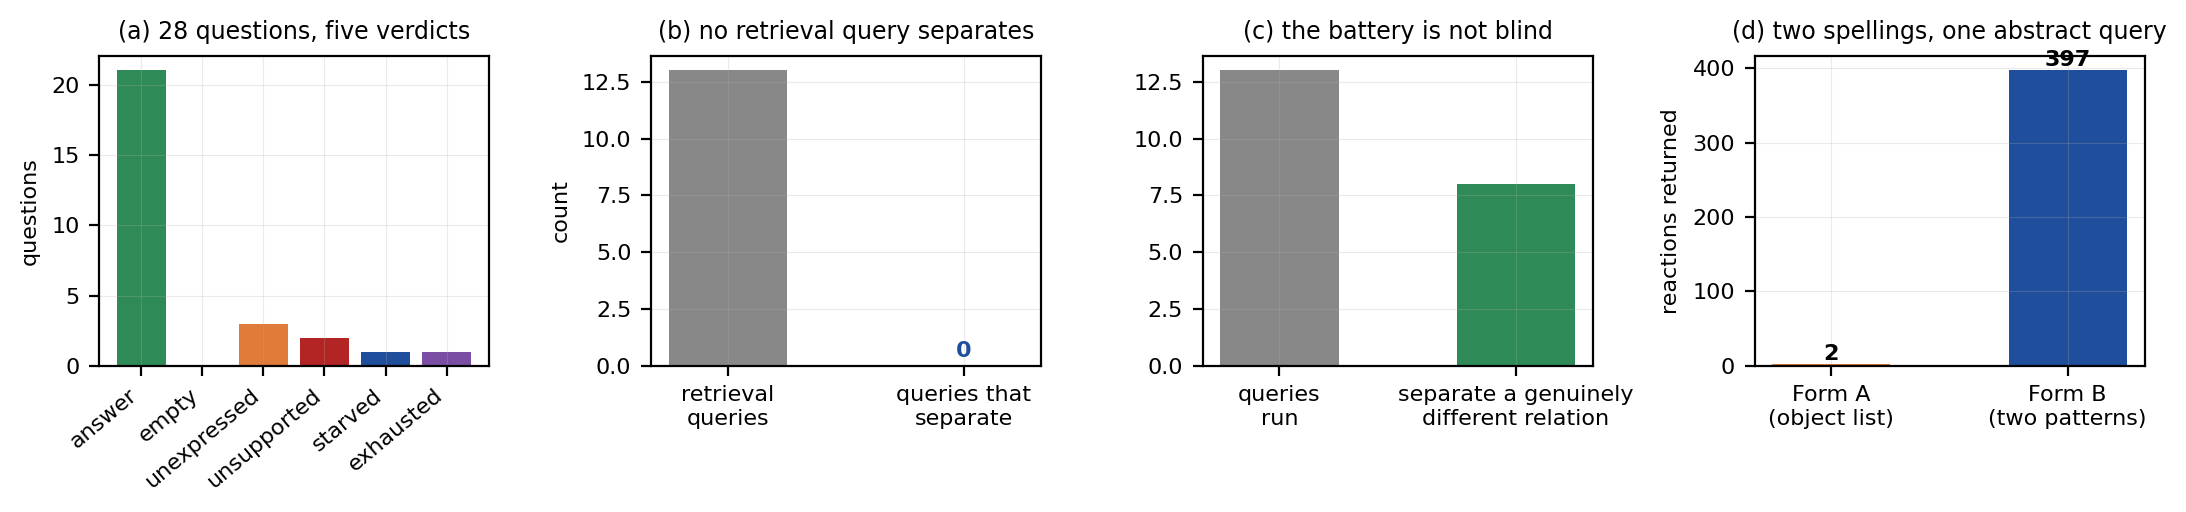
\includegraphics[width=\textwidth]{figures/fig4_verdicts.png}
\caption{\textbf{Verdicts and the expressibility separation.}
\textbf{(a)}~Twenty-eight questions by verdict. Twenty-one are answered and
seven refused, across five distinct outcomes; a system that answered
everything would have an empty defined class.
\textbf{(b)}~Thirteen retrieval query forms run on two independent engines
against two systems with identical triples: none separates them.
\textbf{(c)}~The negative control. The same battery separates a genuinely
different contact relation on $8$ of $13$ queries, so the null result in (b)
is a property of the systems and not of a blind battery.
\textbf{(d)}~The live divergence of \Cref{sec:res-d}: two spellings of one
abstract query returning $2$ and $397$ against the same endpoint on the same
date.}
\label{fig:verdicts}
\end{figure*}

\subsection{Summary of outcomes}

\begin{table}[H]
\centering\small
\caption{Validation summary. Of $58$ reported checks, $57$ are scored and all
pass; $4$ of those are negative controls that must fail on well-formed input
and do, and $1$ further check is recorded non-discriminating and excluded from
the score.}
\label{tab:validation}
\begin{tabular}{@{}llrrr@{}}
\toprule
\textbf{Exp.} & \textbf{Claim checked} & \textbf{Scored} & \textbf{Controls}
& \textbf{Excluded}\\
\midrule
A & \Cref{thm:floor,thm:compose,prop:additive,prop:proportional} & 23 & 1 & 1\\
B & \Cref{thm:separation,cor:attributed} & 9 & 1 & 0\\
C & \Cref{thm:role,thm:trichotomy,prop:saturation,thm:nondegeneracy} & 20 & 1 & 0\\
D & \Cref{obs:status}, the local control & 5 & 1 & 0\\
\midrule
\textbf{total} & & \textbf{57} & \textbf{4} & \textbf{1}\\
\bottomrule
\end{tabular}
\end{table}

We state this explicitly because a table of successes is not by itself
informative. What makes the suite meaningful is that each check was
constructed so that it could have failed, that three are constructed so that
they must fail, and that one was found unable to discriminate and was removed
from the score rather than counted.

% =====================================================================
\part{Scope}
% =====================================================================

\section{What this does not do}
\label{sec:limits}

We state the limits plainly, because several are severe enough that a reader
could otherwise take the paper to claim more than it does.

\paragraph{No experimental validation.} Nothing here has been compared against
a measured hydration structure, a measured direction reversal, a measured
ambient occupancy, or a measured rate. \Cref{thm:trichotomy} is worked from
the qualitative fact that organisms differ in metabolite demand, not from
measured intracellular concentrations. \Cref{cor:oneidentifier} is an
explanation of a documented annotation practice, not a prediction tested
against one.

\paragraph{The powers are declared, not derived.} In
\Cref{sec:questions,tab:questions} the rung powers are literals. Deriving them
from retrieved data --- and answering what a derived power means for a result
set --- is the substantive next step and is not taken here. Until it is, the
ladder demonstrates a \emph{form} of answer on catalysis data rather than a
measured one; measured enzyme parameters cluster well away from physical
limits \citep{barevenn2011}, and reproducing that distribution would be a
real test.

\paragraph{Translation supplies structure.} Converting a record to a contact
graph adds implicit hydrogens, inferred bond orders and a medium the record
never mentions. Unless the translator tags each element as stated or supplied,
a downstream reader cannot tell a recorded fact from a convention. We regard
provenance tagging as a requirement of any serious implementation and have not
implemented it here.

\paragraph{The medium weight is a modelling choice.}
\Cref{eq:mediumweight} is justified by three properties and by reduction to a
chemical potential in the dilute limit, but it is not derived from
\Cref{thm:floor}. A different monotone, floor-bounded function gives the same
theorems with different constants, which is why the suite re-runs every
structural result under four families. Every numerical statement about the
medium is therefore illustrative; the structural statements are not.

\paragraph{No kinetics and no thermodynamics.} The medium bias is not a free
energy: it is a difference of individuation costs. Connecting
$\Delta_\med$ to a reaction free energy \citep{beard2007,noor2013} would be a
substantial and falsifiable next step and is not taken. In consequence ``at what temperature does this
reaction take place'' remains open: the floor is condition-dependent in
principle, but at the categorical depth used here the dependence is
immaterial, and we would rather say so than report a number a laboratory
cannot use.

\paragraph{Fixtures are not the public resources.} Experiments A--C run
against small hand-built stand-ins with the same record shape as the public
sources, not against copies of them. This makes every number reproducible
offline and makes none of them evidence about biology. Only Experiment D
touches a live service.

\paragraph{Capability declarations are asserted.} A source's capability set is
declared by its adapter and is not verified against the service. A wrong
declaration produces a wrong static verdict, and \Cref{thm:static} guarantees
only that the check is decidable, not that the input is true.

\paragraph{One construct is not a general claim.} The ladder is local, pure
and cheap. A construct that had to issue its own requests, or to fail in a way
the six verdicts do not describe, would test the architecture far harder, and
nothing here predicts how that would go.

\section{Conclusion}
\label{sec:conclusion}

A knowledge graph is only as useful as the person who built it and the person
querying it. Both requirements bind, and we have shown an architecture in
which neither binds for an important class of question.

The reason it works is a theorem rather than an engineering trick. An answer
set is a substructure of what was stored, so a question whose answer depends
on a quantity nobody stored has no expression in a retrieval language ---
however good the ontology. We exhibited two systems with identical triples
whose accountability verdicts differ, ran thirteen retrieval query forms
against them on two independent engines without separating them, and confirmed
with a control that the battery is not blind. Storing the weights does not
help, because the quantity that decides is a minimum over subsets and no basic
graph pattern forms one.

What replaces the stored answer is a computation over fetched records. Records
are gathered by a plan whose terms denote results rather than graph patterns,
translated into contact graphs, and stencilled with a ladder. Because the
stencil asks only for a separation cost, it applies to records whose schema
has no notion of the thing being asked --- which is how one queries items one
cannot model. The solvent's role becomes a comparison of two boundaries rather
than a curator's annotation; a reaction's direction becomes a trichotomy on
one inequality, so that one identifier can correctly name a process running
opposite ways in two organisms.

The framework refuses. Seven of twenty-eight questions are declined, each
naming a blocker and a remedy, and refusal is enforced structurally: no
verdict but \vans{} may carry a payload. A framework that classifies
everything has an empty defined class.

Two results came from tests written to be capable of failing. A one-sided
sweep of the direction trichotomy never reached its third case, and the reason
turned out to be a saturation bound we had not anticipated: flooding a product
cannot reverse a chain, because the attainable bias stops at
$-\log(1+\tau/\mu_0)$, while depleting a reactant is unbounded. And the
counter-intuitive claim that control lies at the strongest rung survives only
under an additive parametrisation; under proportional improvement the
sensitivity is flat, at machine zero over five thousand ladders. We report
both because a suite written to pass would have hidden them.

What remains is the measurement. The powers here are declared and not derived
from kinetics, no number has been checked against a laboratory, and the
translation from record to graph supplies more than it states. Those are the
next experiments, and they are the ones that would make the architecture a
scientific instrument rather than a well-founded proposal.

% =====================================================================
\section*{Reproducibility}
\addcontentsline{toc}{section}{Reproducibility}

All experiments are in \texttt{validation/}. Running
\texttt{python exp\_a\_ladder.py}, \texttt{exp\_b\_expressibility.py},
\texttt{exp\_c\_questions.py} and \texttt{exp\_d\_divergence.py} reproduces
every number quoted, writing per-experiment JSON to \texttt{results/};
\texttt{make\_figures.py} regenerates every panel from those files. The
reference kernel is \texttt{kernel/ladder.py} and \texttt{kernel/plan.py};
the fixtures are \texttt{fixtures/corpus.py}. Experiments A--C require no
network. Experiment D contacts a public SPARQL endpoint and degrades to its
local control if the service is unavailable.

% =====================================================================
\bibliographystyle{plainnat}
\bibliography{references}

\end{document}
